\documentclass{article}
\usepackage[utf8]{inputenc}
\usepackage{caption}
\usepackage[margin=1in]{geometry}
\usepackage{graphicx}
\graphicspath{ {Images/Assignment2} }


\title{Assignment 2: CART}
\author{Lorenzo Meninato}
\date{March 2018}

\begin{document}

\maketitle

Do "illegitimate" factors, such as gender, race, ethnicity, and nationality, have a substantial impact on whether or not defendants of capital crimes are charged with the death penalty? If these factors do have an impact, how much of an impact do they have, and which factors have the largest impact? This question would be of policy interest to various parties, such as lawmakers, politicians, and social justice organizations. 

\section{Introduction}
In the United States, there is both a state criminal justice system and a federal criminal system. The data come from the federal system during the Clinton Administration (1993-2001), and includes all homicide cases for which it was legally permitted to seek the death penalty. The data were collected to consider federal death penalty charging practices with the goal of possible subsequent reform. 

\begin{figure}[!htb]
    \centering
    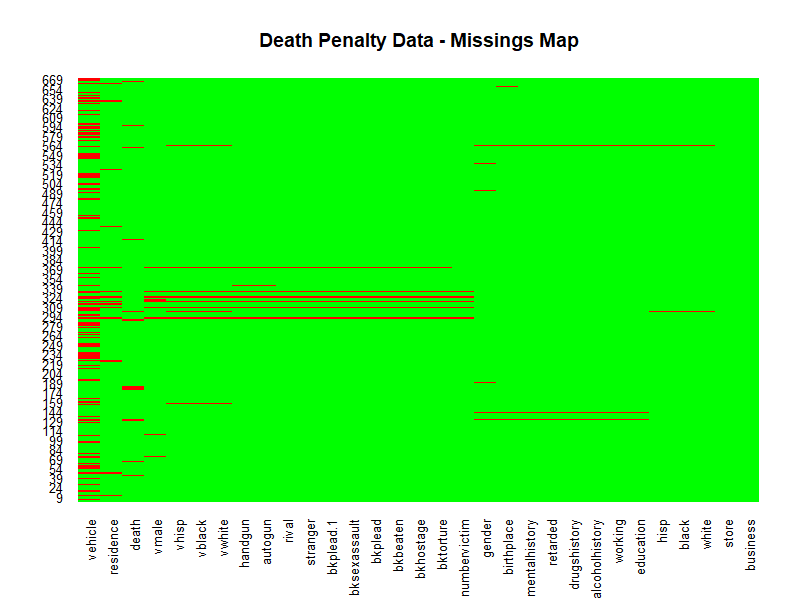
\includegraphics[scale=0.75]{/missing1.png}
    \caption{Map of missing data.}
    \label{mis1}
\end{figure}

Figure \ref{mis1} shows that there are many missing observations. In particular, many observations are missing for whether or not a vehicle was involved (188), and a few observations are missing many characteristics, from the victims race, to details about the crime. In terms of my preemptive data manipulations, I have to consider the trade-off between removing many observations, and thus reducing my sample size, and introducing bias through working with an incomplete dataset. Either way some statistical power will be lost, but I will try to strike a balance between bias and statistical power. Since I am regressing death on various factors, it makes little sense to include observations for which whether or not the defendant was killed is a missing observations (occurs in 23 cases). Further, for the key factors central to my research questions, such as gender, race, and education, if those factors are missing, the statistical analysis will be less capable of answering the question of how those factors impact the probability of a death penalty sentence. Jointly, there are only 34 rows that are missing any of those factors I deem "key" to answering the research question. Thus I can still analyze how those factors impact death sentence probability with a dataset of 635 observations, only 34 observations less than the original dataset of 669 observations. I considered using more advanced data imputation techniques, such as considering the values of neighboring observations, and imputing the averaged values onto the missing points, but since my dataset is still quite large after removing those observations, I felt this would only artificially reduce variance, and increase the bias of my results. Even more advanced techniques like multiple imputation methods from the "mice" library would still introduce this problem. However, completely removing all observations with any missing data would have shrunk my dataset to two-thirds the size. This seemed like another extreme that would have reduced the statistical power of the data. Since the dataset is not that large, this did not seem appropriate. However, I still have a significant number of missing observations for other variables, fortunately, many of the missing observations are clustered within the same row, so I can remove the rows containing these missing values without decimating the dataset.

My compromise is to completely remove the vehicle column, then omit any rows with missing values. Even if I were to impute in the missing values for the vehicle column, this would not be recommended since there are so many missing observations. I only lose 74 observations doing this, and then I do not have to worry about handling missing data within CART. It is generally better to allow CART to handle missing data if data appears to be completely at random (for evidence of this, note how in Figure 1 there are long horizontal lines, and the missing observations are clustered around the middle. The missing data for the vehicle column appear to be fairly random.), but judging from my missing data maps this does not seem to be the case. So in this case, imputing over so many observations will likely fail \footnote{Inconveniently this is when this would be most useful.}. If there were fewer missing observations, imputation would be a better approach. Thus using surrogate variables would likely lead to an unreliable correspondence between the results and the data. 

In summary, I will attempt to resolve the missing data issue by dropping the vehicle column, and then removing all rows with missing observations.

\begin{figure}[!htb]
    \centering
    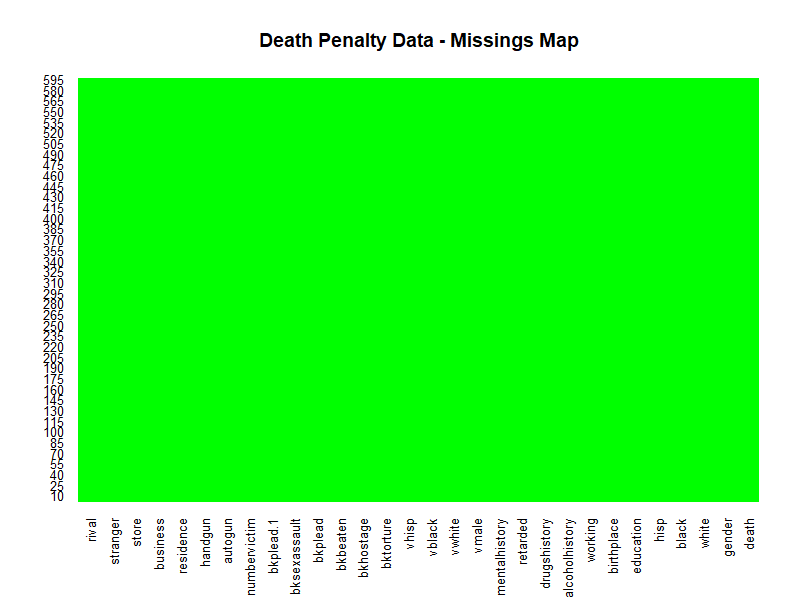
\includegraphics[scale=0.75]{/missing2.png}
    \caption{Map of missing data after transformation.}
    \label{mis2}
\end{figure}

Our new dataset now contains no missing observations. Further, since our dataset contains 30 variables, 1 of which is a tertiary variable (education), I have to codify it as a factor variable in R, otherwise the CART algorithm might treat it is a continuous variable, and the arbitrary divisions between the factor levels would no longer be arbitrary \footnote{So coding no education as a 2 rather than a 5, for instance, would yield different results. This is of course undesired.}. The other variables are either binary or numeric (number of victims). This is checked to guarantee that binary variables are not treated as continuous when I apply the algorithm \footnote{See appendix for code.}. If this were not checked, the results would be more tenuous. 

\newpage

\section{Univariate Analysis}

As a sanity-check, we can see that the number of victims is always at least 1 (it would not make sense for there to exist crimes without victims). Unsurprisingly there is a right-skewed distribution of the number of victims. It will be interesting to see how the number of victims impact the probability of death penalty sentence in the bivariate statistics analysis. For instance, we could see that each additional victim increases the death sentence probability, or it is possible that there is no relationship. I explore this in the bivariate analysis of the data. If there is a relationship, we would expect this to be communicated in the results of the regression tree. 

\begin{figure}[!htb]
    \centering
    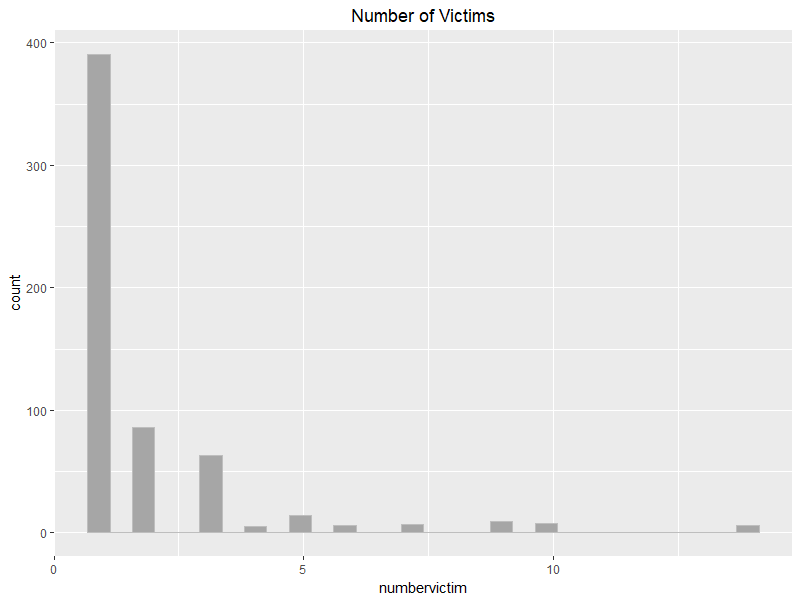
\includegraphics[scale=0.6]{/nvictims1.png}
    \caption{Number of Victims per Crime.}
    \label{nv1}
\end{figure}

\newpage

Most of the crimes were committed by fairly uneducated people. Only about a third of defendants had at least a high school degree. There does seem to be a significant amount of uncertainty about this however, since over half the observations had an unknown level of education. This might be important in terms of determining splits in the regression trees, since splits based on education might be highly uncertain, since so much of the data is weighted towards the unknown factor level. Although I am no expert in the relevant subject-matter, but one could hypothesize that more educated suspected murderers could face more lenient sentences at greater rates since the jury might find them more capable of re-integrating into society. Of course, perhaps there is an even stronger counterargument that a marginalized individual who had a very poor education should be treated more leniently, precisely because the systemic disadvantage such an individual would have faced. This could have given key insights into whether education influences sentences or not. Either way, going forward I must take into consideration the uncertainty embedded in this variable. 

\begin{figure}[!htb]
    \centering
    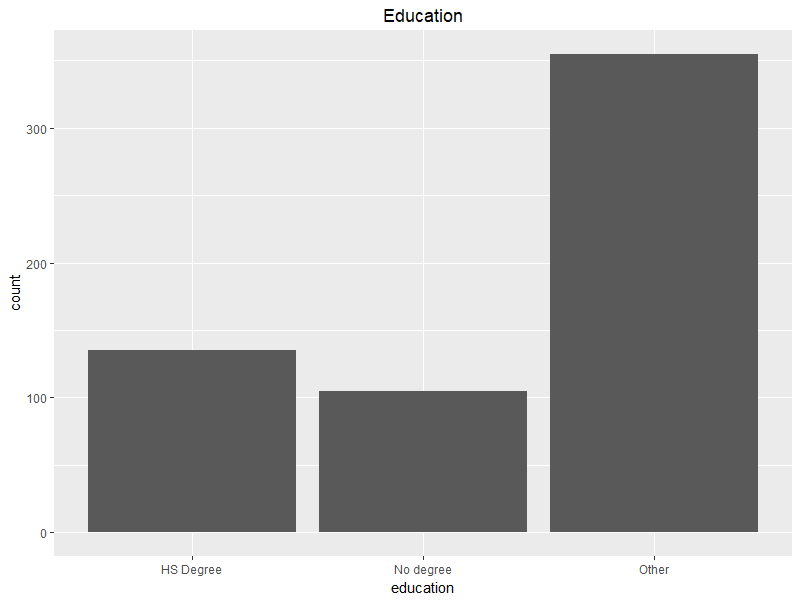
\includegraphics[scale=0.6]{/education1.png}
    \caption{Distribution of defendant's education.}
    \label{ed1}
\end{figure}

The majority of capital crimes were committed by men (574 vs. 21 observations) and about 24\% of crimes overall received the death sentence. The racial composition of the defendants skewed towards black (48\%) and Hispanic (27\%) ethnicities. Further, it will be interesting to see how sentencing is impacted by differences in ethnicity between the perpetrator and the victim. There were more female victims (15\%) than female perpetrators (3.5\%). It will be interesting to see if a man killing a woman results in more severe punishment than otherwise. I would also expect that mentally disabled defendants would receive the death penalty less often. For the "before killing" variables, if the case involved some "before killing" act, I would expect the death sentence probability to increase. All the proportions are listed in Table \ref{table:props} \footnote{Code is in the appendix.}.

\newpage

\section{Bivariate Analysis}

There do not seem to be any clear trends with respect to the relationship between death sentence probability and education. The proportions confirm this: 31.8\% HS degree,  29.5\% no HS degree, 19.7\% other. The death sentence probability does seem to be statistically significantly less for those with an unknown education, thus having had better data the results might be able to be much stronger. 

\begin{figure}[!htb]
    \centering
    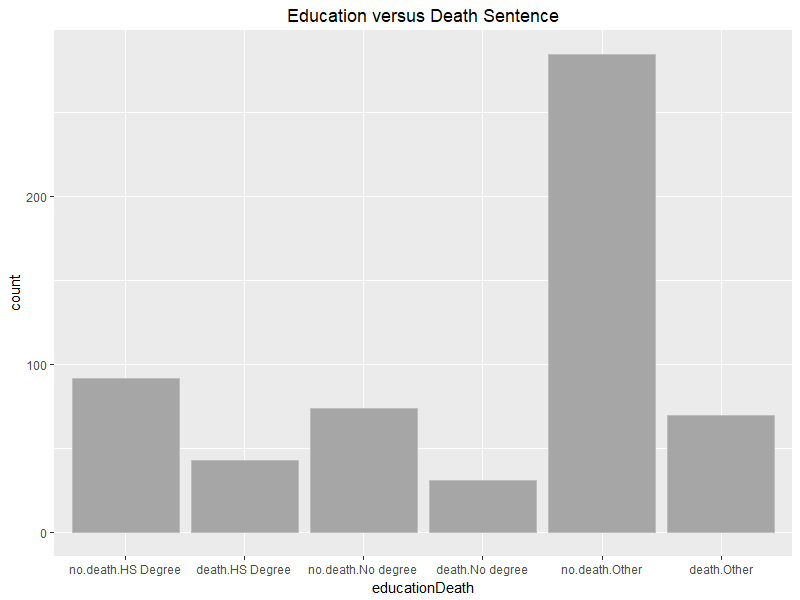
\includegraphics[scale=0.6]{/education2.png}
    \caption{Interaction between Education and Punishment}
    \label{ed2}
\end{figure}

A Level I analysis reveals that the number of victims per crime does have a significant effect on the probability of a death sentence. I can then quickly compute the an estimate of the death penalty sentence probability based on the number of victims. As expected, Figure \ref{nv3} shows that the linear regression line trends upwards, so the more victims, the greater the chance of a death sentence. 

\begin{figure}[!htb]
    \centering
    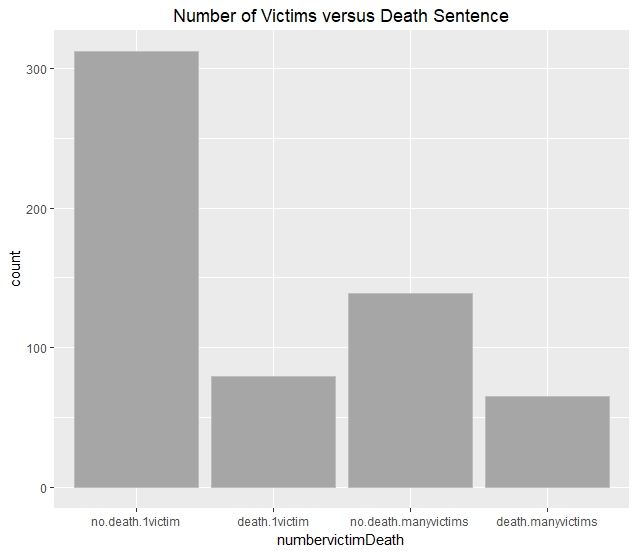
\includegraphics[scale=0.6]{/nvictims2.png}
    \caption{Interaction between Number of Victims and Punishment}
    \label{nv2}
\end{figure}

Examining the relationships between the race and death sentence probability, I find that a cursory glance at the summary statistics \footnote{Code available in the appendix (necessary to combine variables in certain ways to table data).} finds that over 56 observations, 39\% of black defendants with white victims received the death penalty, while over 232 observations only 19.8\% of black defendants with crimes against non-whites received the death penalty. This difference could provide substantial evidence that illegitimate factors do play a role death penalty sentences. Interestingly, I do not find a similar result crimes committed against whites by Hispanics (about 11\% more death sentences granted for Hispanic crimes against non white victims). For crimes by whites against whites, about 37\% of defendants were granted the death penalty, while in 9 cases of white crimes against non-white victims, only 22\% of defendants were granted the death penalty. In summary, only the data of black-on-white crime appears to support the hypothesize that blacks were granted the death penalty at greater frequencies. 

\begin{figure}[!htb]
    \centering
    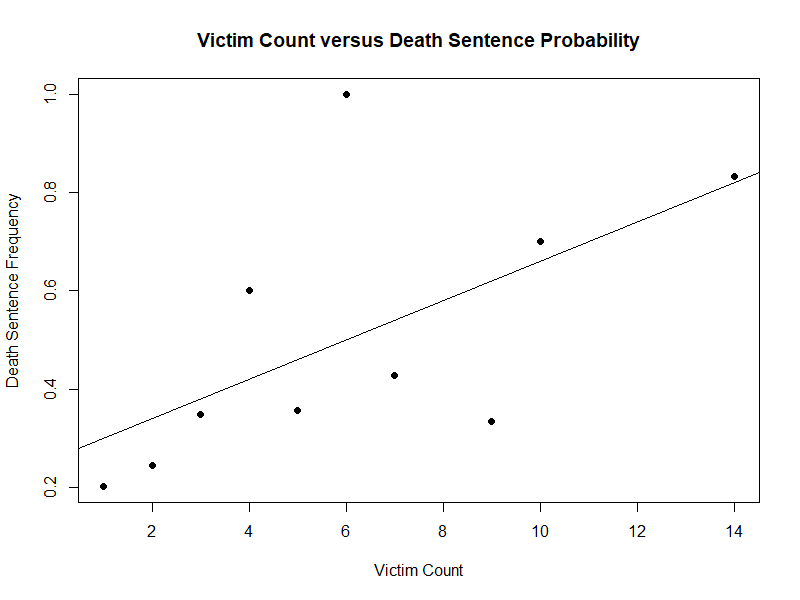
\includegraphics[scale=0.6]{/nvictims3.png}
    \caption{Interaction between Number of Victims and Punishment}
    \label{nv3}
\end{figure}


Due the inherent complexity in a dataset with so many variables, it is pointless to try understand all the possible interactions between variables. In fact, because of that complexity, machine learning algorithms will quite possibly be more useful than conventional statistical techniques. So certain variables that I have not analyzed more thoroughly, like the "before killing" variables, gun and store variables, etc. might end up playing a larger role than an initial Level I analysis might imply. This is might only be possible in an algorithmic sense, since even simply thinking about all the possible covariances and correlations between 30 or more variables would consume an inordinate amount of a researcher's time. 

It would be prudent to consider the possible risks of overfitting the data to the model. By separating our dataset into training and test data we can check for overfitting by running the test data through the outputted regression tree. One possibility for reducing overfitting is to increase the cost complexity of the CART model. The penalty for complexity is a function of the number of terminal nodes in the model. However, the bias-variance trade-off reappears under the true model perspective (when operating at Level II analysis). Larger trees will have fewer classification errors, which implies less bias, but the same tree will have fewer cases to check, and thus more tree instability, thus a greater variance. I can tweak the $cp$ parameter when minimizing $$R_{cp} (T) \equiv R(T) + cp*|T|*R(T_1)$$ to find a suitable trade-off between bias and variance. 

However, before implementing the CART model, I must justify the use of statistical inference with CART. For operating at a Level II analysis, the key assumption is that the data are realized from a join probability distribution of subject-matter interest, where $Y$ and $X$ are random variables. As discussed in Chapter 1 of the text, this is rarely possible, instead we can treat CART as an attempt to estimate an approximation of the true response surface. While the data does cover all cases where it was legal to seek the death penalty, in which case we would expect the data to be drawn from the appropriate distribution, the nature of the data is that it is quite sparse, since at best there are about 670 observations, and after splitting the data into training, evaluation, and test data, statistical inference would be quite limited. But apart from the various limitations, I can still tentatively proceed with a Level II analysis. 

\newpage


\section{CART Model}
I applied the $rpart()$ model to the data. In order to tune the structure of the tree, I manipulate the $cp$ parameter. My cost ratio target is that false negatives (no death sentence is predicted, when death sentence was given) are preferred to false positive (death sentence is predicted, when no death sentence was given) by at least 10 to 1. 
I use the Gini classification loss function since the entropy function is more computationally intensive and I did not receive better results by using it.

\begin{figure}[!htb]
    \centering
    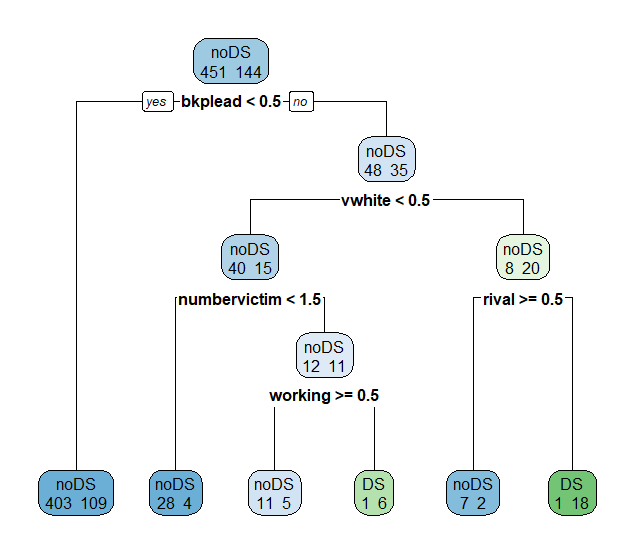
\includegraphics[scale=0.6]{/tree1.png}
    \caption{CART model with cp=0.01 and loss matrix with 3:1 ratio (N=595).}
    \label{tree1}
\end{figure}

The quality of the fit of this model was quite high (see Table \ref{table:tree1}). The model error was relatively high (0.83), but this is the inherent trade-off between setting a cost ratio that heavily emphasizes avoiding unfairly sentencing an individual to death. I think this target is necessary, given the subject matter, since there is a strong ethical argument that it is preferred for many criminals to serve life sentences, even if they "deserve"\footnote{If one assumes that a criminal \textit{can} deserve the death penalty.} the death penalty, if it results in an innocent defendant not being condemned to death. 

\begin{figure}[!htb]
    \centering
    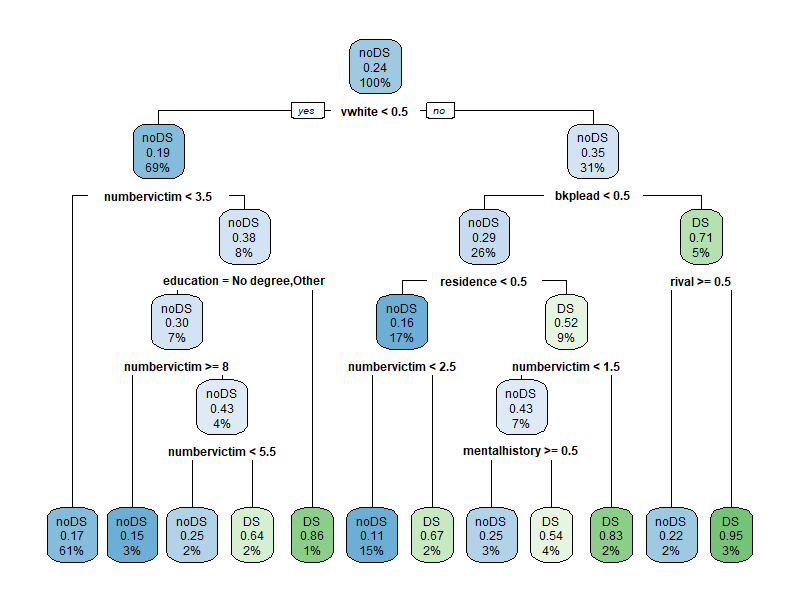
\includegraphics[scale=0.6]{/tree2.png}
    \caption{CART model with cp=0.01 and default cost ratio target (N=595).}
    \label{tree2}
\end{figure}

I found that the $cp$ value of 0.01 worked fairly well, since at lower $cp$ values the used more variables to determine node splits, but it ended up splitting nodes through the "victim number" variable many times. Notice how in Figure \ref{tree2} the number of victims is pinned down 3 times along the left branch. This type of structure did not seem particularly illuminating. I found that the parameters set in \ref{tree1} managed to find a balance between simplicity and informativity.

\begin{table}[!htb]
\centering
\label{table:tree1}
\begin{tabular}{|l|ll|ll|}
\hline
          & Classify as no DS & Classify as DS & Model error &  \\
          \hline
no DS     & 449               & 2              & 2/551       &  \\
DS        & 120               & 24             & 120/144     &  \\
\hline
Use error & 120/569           & 2/26           & 122/595     &  \\
\hline
\end{tabular}
\caption{CART confusion table for classifying sentence for capital crimes with 3:1 loss ratio.}
\end{table}

Of course, even with a given cost ratio, CART performance cannot be reduced to a single number. Some might prefer that that the tree make sense from a subject matter perspective. It can be difficult to form a tree that "makes sense" for this dataset, since even with variables about the case itself, like the "before killing" variables or "number of victims", it is not clear how such variables would interact with each other. Therefore, there is no obvious subject matter knowledge that informs the structure of the tree. Others might care solely about the classification accuracy of the tree. The accuracy can be obtained from the confusion table, but there are several evaluation metrics, like explanation, classification, and forecasting, that can be optimized. 



\section{Conclusion}
Given how the data is relatively sparse, even my relatively weak CART results can be useful to data analysts. This is a bit trickier since I am working at a Level II, but were there more data, even very strong CART results would be irrelevant, since other techniques would likely be more informative. This seems to be the main complication of using CART for statistical inference. 

There appear to be three main variables associated with a death penalty sentence: whether or not the victim pleads for mercy, whether or not the victim is white, and the number of victims. Using a CART model that imposes a penalty for false positives, when the victims of a crime was white, they were much more likely to receive a death penalty sentence. 
While I found no evidence that supports that non-whites are statistically significantly more likely to be given the death than whites for the same crime, crimes committed against whites were more likely to result in a capital charge than equivalent crimes against non-whites. This appears to be an illegitimate factor that perhaps should be addressed with policy initiatives, through either treating crimes against non-whites more seriously or through diverting resources away from prosecuting crimes against whites. This result could possibly be explained by families of white victims having either more judicial or financial resources to prosecute defendants of any background, in order to ensure that the defendant receives a death sentence. 




\section{Appendix}

\begin{table}[!htb]
\centering
\begin{tabular}{rrl}
  \hline
 & Proportion & Variable Name \\ 
  \hline
  1 & 0.24 & death \\ 
  2 & 0.96 & gender \\ 
  3 & 0.18 & white \\ 
  4 & 0.48 & black \\ 
  5 & 0.27 & hisp \\ 
  6 & 0.89 & birthplace \\ 
  7 & 0.79 & working \\ 
  8 & 0.09 & alcoholhistory \\ 
  9 & 0.20 & drugshistory \\ 
  10 & 0.06 & retarded \\ 
  11 & 0.18 & mentalhistory \\ 
  12 & 0.85 & vmale \\ 
  13 & 0.31 & vwhite \\ 
  14 & 0.42 & vblack \\ 
  15 & 0.27 & vhisp \\ 
  16 & 0.05 & bktorture \\ 
  17 & 0.21 & bkhostage \\ 
  18 & 0.18 & bkbeaten \\ 
  19 & 0.14 & bkplead \\ 
  20 & 0.05 & bksexassault \\ 
  21 & 0.14 & bkplead.1 \\ 
  22 & 0.37 & autogun \\ 
  23 & 0.61 & handgun \\ 
  24 & 0.25 & residence \\ 
  25 & 0.11 & business \\ 
  26 & 0.09 & store \\ 
  27 & 0.32 & stranger \\ 
  28 & 0.55 & rival \\ 
   \hline
\end{tabular}
\caption{List of frequencies for each variable.}
\label{table:props}
\end{table}


\newpage

\begin{verbatim}
library(rpart)
library(rpart.plot)
library(ipred)
library(xtable)

load("~/R/MLDeathPenalty.rdata") #loading dataset

summary(DeathPenalty)
copy = na.omit(DeathPenalty)

require(Amelia)
missmap(DeathPenalty, main="Death Penalty Data - Missings Map", col=c("red", "green"),
        legend=FALSE)
#library(mice)
#tempData <- mice(DeathPenalty,m=5,maxit=50,meth='pmm',seed=500)

missing = is.na.data.frame(DeathPenalty[,c(1,2,3,4,5,7)])
missing = as.data.frame(missing)
whichMissing = which((missing$black | missing$white | missing$death | missing$gender | missing$hisp | missing$birthplace) != FALSE)

copyDP = DeathPenalty[-whichMissing,]
missmap(copyDP, main="Death Penalty Data - Missings Map", col=c("red", "green"),
        legend=FALSE)
copyDP = subset(copyDP, select = -c(vehicle))

copyDP = na.omit(copyDP)
missmap(copyDP, main="Death Penalty Data - Missings Map", col=c("red", "green"),
        legend=FALSE)
copyDP$education = as.factor(copyDP$education)
levels(copyDP$education) = c("HS Degree", "No degree", "Other")


x= rep(0,30)

for (i in c(1:30)){
  x[i] = length(unique(copyDP[,i]))
}
#confirms that all variables are binary except 2. 

factors = which(x == 2)
factorCopy = copyDP
factorCopy[,factors] <- lapply(factorCopy[,factors], factor)
summary(factorCopy)
#for nice univariate summary statistics

proportions = rep(0,ncol(factorCopy))

for (i in 1:length(proportions)){
  proportions[i] = substr(as.character(summary(factorCopy)[2,i]), start =3, stop = 6)
}
proportions = as.integer(na.omit((as.integer(proportions))))/nrow(factorCopy)
#proportions for binary variables
namesList = names(factorCopy)
namesList = namesList[-c(6, 23)]
props = data.frame(proportions, namesList)
#proportions
xtable(props)

library(ggplot2)

ggplot(copyDP, aes(numbervictim))+
  geom_histogram(col="grey", fill ="grey65")+
  theme(plot.title = element_text(hjust = 0.5))+
  labs(title="Number of Victims")

ggplot(copyDP, aes(education))+
  geom_bar()+
  theme(plot.title = element_text(hjust = 0.5))+
  labs(title="Education")


factorCopy$educationDeath = rep(0,nrow(factorCopy))
levels(factorCopy$death) = c("no.death", "death")

factorCopy$educationDeath = with(factorCopy, interaction(factorCopy$death, factorCopy$education))
xtable(table(factorCopy$educationDeath))

ggplot(factorCopy, aes(educationDeath))+
  geom_bar(col="grey", fill ="grey65")+
  theme(plot.title = element_text(hjust = 0.5))+
  labs(title="Education versus Death Sentence")

#death proportions: 31.8% HS degree,  29.5% no HS degree, 19.7% other

factorCopy$manyVictims = factor(ifelse(factorCopy$numbervictim == 1, "1victim", "manyvictims"))
factorCopy$numbervictimDeath = with(factorCopy, interaction(factorCopy$death, factorCopy$manyVictims))

ggplot(factorCopy, aes(numbervictimDeath))+
  geom_bar(col="grey", fill ="grey65")+
  theme(plot.title = element_text(hjust = 0.5))+
  labs(title="Number of Victims versus Death Sentence")

factorCopy$numbervictimDeath2 = with(factorCopy, interaction(factorCopy$death, factorCopy$numbervictim))
nvictimDeathProb = c(79/(312+79), 21/(65+21), 22/(41+22), 3/(2+3), 5/(9+5), 6/6, 3/(4+3), 3/(6+3), 7/(3+7), 5/(5+1))
victimcount = c(1,2,3,4,5,6,7,9,10,14)
plot(victimcount, nvictimDeathProb, pch = 16, main = "Victim Count versus Death Sentence Probability", xlab = "Victim Count", ylab = "Death Sentence Frequency")
abline(lm(nvictimDeathProb ~ victimcount))

levels(factorCopy$black) = c("notBlack", "Black")
levels(factorCopy$vwhite) = c("notwhiteV", "whiteV")
factorCopy$BlackWhite = with(factorCopy, interaction(factorCopy$black, factorCopy$vwhite, factorCopy$death))
xtable(table(factorCopy$BlackWhite))

levels(factorCopy$hisp) = c("notHisp", "Hisp")
levels(factorCopy$vwhite) = c("notwhiteV", "whiteV")
factorCopy$HispWhite = with(factorCopy, interaction(factorCopy$hisp, factorCopy$vwhite, factorCopy$death))
xtable(table(factorCopy$HispWhite))

levels(factorCopy$white) = c("notWhite", "White")
levels(factorCopy$vwhite) = c("notwhiteV", "whiteV")
factorCopy$WhiteWhiteV = with(factorCopy, interaction(factorCopy$white, factorCopy$vwhite, factorCopy$death))
xtable(table(factorCopy$WhiteWhiteV))
#Tables for information about crimes against white victims. 

load("~/R/MLDeathPenalty.rdata") #loading dataset
copyDP = DeathPenalty
copyDP = subset(copyDP, select = -c(vehicle))
copyDP = na.omit(copyDP)
copyDP$education = as.factor(copyDP$education)
levels(copyDP$education) = c("HS Degree", "No degree", "Other")
copyDP$death = as.factor(copyDP$death)
levels(copyDP$death) = c("noDS", "DS")


regTree = rpart(death~. , data = copyDP, cp = 0.01)
rpart.plot(regTree)

regTree = rpart(death~., data = copyDP, parms=list(loss=matrix(c(0,3,1,0),2,2,byrow=TRUE)), cp = .01)
rpart.plot(regTree, extra = 1)

pred = predict(regTree, copyDP, type = "class")
table(copyDP$death, pred)



\end{verbatim}

\end{document}
